\documentclass[letterpaper,9pt,onecolumn,twoside,]{pinp}

%% Some pieces required from the pandoc template
\providecommand{\tightlist}{%
  \setlength{\itemsep}{0pt}\setlength{\parskip}{0pt}}

% Use the lineno option to display guide line numbers if required.
% Note that the use of elements such as single-column equations
% may affect the guide line number alignment.

\usepackage[T1]{fontenc}
\usepackage[utf8]{inputenc}

% pinp change: the geometry package layout settings need to be set here, not in pinp.cls
\geometry{layoutsize={0.95588\paperwidth,0.98864\paperheight},%
  layouthoffset=0.02206\paperwidth, layoutvoffset=0.00568\paperheight}

\definecolor{pinpblue}{HTML}{18AF67}  % imagecolorpicker on blue for new R logo
\definecolor{pnasbluetext}{RGB}{101,0,0} %



\title{Variación de la altura de Vismia Macrophylla y Jacaranda Copaia a través
de diferentes estados de sucesión de un bosque húmedo tropical de
acuerdo con sus hábitos de crecimiento}

\author[a]{Camilo Cruz Sanchez}
\author[a]{Yonatan Moran Ruano}
\author[a]{Elkin Vanegas Vargas}
\author[a]{Cristian Gañan Tapasco}

  \affil[a]{Departamento de ciencias forestales, Univeridad Nacional de Colombia,
Medellín}

\setcounter{secnumdepth}{0}

% Please give the surname of the lead author for the running footer
\leadauthor{Sanchez-Moran-Vanegas-Gañan}

% Keywords are not mandatory, but authors are strongly encouraged to provide them. If provided, please include two to five keywords, separated by the pipe symbol, e.g:
 \keywords{  Vismia Macrophylla |  Jacaranda Copaia |  Sucesión |  Radiación | Perturbación }  

\begin{abstract}
Entender el comportamiento de variables como altura y radiación es de
vital importancia para analizar las dinámicas de regeneración que un
ecosistema ha tenido de acuerdo con las perturbaciones particulares que
presenta. En este informe se analizan aspectos como el crecimiento y
distribución de dos especies (Vismia Macrophylla y Jacaranda Copaia), en
4 parcelas con diferentes estados de sucesión; dicho análisis se realiza
de acuerdo con los hábitos de crecimiento de cada una de las especies.
Se aplica el modelo Michaelis Menten con un RSE de 2.70 y un AIC de
876.90 para explicar el crecimiento de estas especies y la forma como
varía su altura relacionado con el cambio en el estado de sucesión del
bosque, obteniendo relaciones significativas entre la altura de las
especies, el estado de sucesión y categoría de vegetación (brinzales, latizales y fustales) . De la misma forma por medio del
análisis del porcentaje de radiación realizado mediante el software
ImageJ se busca mostrar la disminución de disponibilidad de luz que
atraviesa el dosel obteniendo la mayor cantidad de luz (17,38\%) en la
parcela 4 que presenta un estado de sucesión SS1 y una menor cantidad de
luz (8,92\%) en la parcela 2 con un estado de sucesión SS3, demostrando
así dicha hipótesis.\\
\end{abstract}


% initially we use doi so keep for backwards compatibility
% new name is doi_footer
\doifooter{Depertamento de ciencias forestales}

\pinpfootercontents{Ecología Forestal}

\begin{document}

% Optional adjustment to line up main text (after abstract) of first page with line numbers, when using both lineno and twocolumn options.
% You should only change this length when you've finalised the article contents.
\verticaladjustment{-2pt}

\maketitle
\thispagestyle{firststyle}
\ifthenelse{\boolean{shortarticle}}{\ifthenelse{\boolean{singlecolumn}}{\abscontentformatted}{\abscontent}}{}

% If your first paragraph (i.e. with the \dropcap) contains a list environment (quote, quotation, theorem, definition, enumerate, itemize...), the line after the list may have some extra indentation. If this is the case, add \parshape=0 to the end of the list environment.


\hypertarget{introduccuxedon}{%
\section{Introduccíon}\label{introduccuxedon}}

Colombia presenta una alta diversidad biológica, amenazada por la
intensa presión antrópica que envuelve la deforestación, la
fragmentación y los cambios en el uso del suelo, causados principalmente
por actividades ganaderas y agrícolas.\citep{salas} Las áreas que se
recuperan de la perturbación, donde se ha practicado principalmente la
agricultura de subsistencia de roza y quema, y zonas de pastura para la
ganadería, generan un aumento de los bosques secundarios\citep{hammer}
que han venido presentando una regeneración a través del tiempo.

La Regeneración del ecosistema hace parte de un proceso dinámico en el
cual nuevos individuos entran a hacer parte de la población reproductora
a medida de que otros mueren por medio de un proceso natural
\citep{pulido}, dando así paso a nuevas especies más prósperas en las
condiciones que surgen a partir del cambio de vegetación y variables
climáticas. La incidencia de las prácticas forestales o agrícolas suele
alterar los parámetros de regeneración del bosque ya que esto altera
condiciones esenciales para la vida de ciertas especies cambiando así la
evolución natural del bosque \citep{pulido}.

Para el estudio de la regeneración o sucesión ecológica en el bosque
húmedo tropical de La Reserva Natural Hacienda San Pedro ubicada en
la cuenca media del río Magdalena se definen cuatro estados sucesionales
de crecimiento del bosque: SS1: sucesión en edad de 0-5 años, con área
de 30 ha, presencia de pastos, escasa vegetación arbórea y donde
predominó la actividad ganadera; SS2: sucesión en edad de 10-13 años con
vegetación arbórea, con área de 50 ha, con presencia de helechos y
dominio de especies heliófilas de rápido crecimiento, con suelo
anteriormente usado en actividades agrícolas; SS3: sucesión con edad de
18-20 años, con área de 40ha, con algunos árboles de altura mayor a 30m
y un dosel más cubierto, con presencia de epífitas y especies tolerantes
a la sombra y con suelo antes usado en actividades ganaderas; SS4:
sucesión avanzada con edad mayor a 50 años, con área de 180 ha, con
grandes árboles y dosel cubierto, con pocos claros y presencia de
epífitas y bromelias y con presencia de bosque anteriormente sometido a
tala selectiva \citep{sala}.

En esta reserva se realizó un levantamiento de datos por medio de 4
parcelas ubicadas según las condiciones topográficas y logísticas, donde
se tuvieron en cuenta dos especies, la primera \emph{Jacaranda Copaia}
que es un árbol grande de hasta 35 m de altura que vive mejor a una
altura de 0 a 1000 msnm, siendo este de tipo heliófita y una especie
pionera en la regeneración de bosques \citep{tapia}, de la cual se
encontraron muy pocos individuos en todas las parcelas; y la segunda
\emph{Vismia Macrophylla}, árbol o arbusto característico de lugares en
barbecho, enrastrojados o áreas de pastos cercanas a bosques
fragmentados, de tipo Heliófita \citep{leza}, puede llegar a medir hasta
12 m de altura, presente más comúnmente entre los 10 a 700
msnm\citep{vismia}. Con dichas especies se realizó una comparación entre
los estados sucesionales de crecimiento, estados de vegetación y el cambio en la altura de
estas dos especies en las diferentes parcelas por medio de los modelos
Weibull y Michaelis Menten.

Las radiación que llega a un determinado lugar influye en numerosos
procesos fisiológicos, reproductivos de plantas, y afecta de forma muy
significativa el funcionamiento general del ecosistema. Los rasgos de la
radiación que tienen relevancia ecológica y evolutiva son: la
intensidad, la calidad, la direccionalidad, y la distribución en el
tiempo y en el espacio. Además, la luz es el factor abiótico más
variable en el tiempo y en el espacio, el análisis de esta variabilidad,
así como sus causas y consecuencias , supone una de las mejores
aproximaciones al estudio de la luz como un factor ecológico y evolutivo
muy importante. \citep{vallares} Es por lo que mediante un análisis de
porcentaje de radiación que pasa a través del dosel realizado con el
software ImageJ por medio de fotos tomadas en medio del dosel dentro de
las parcelas, se mostró la disminución en la disponibilidad
de luz a medida que la regeneración del bosque es más avanzada, con
esto se analizó el comportamiento en la cantidad de individuos encontrados
en cada parcela de las especies mencionadas anteriormente según sus
hábitos de crecimiento y el gremio ecológico a que pertenecen.

Con todo esto se espera responder cómo varía la altura de Vismia
Macrophylla y Jacaranda Copaia a través de los diferentes estados de
sucesión y categoria de vegetación en un bosque húmedo tropical de acuerdo con sus hábitos de
crecimiento.

\hypertarget{materiales-y-muxe9todos}{%
\section{Materiales y métodos}\label{materiales-y-muxe9todos}}

\hypertarget{localizaciuxf3n-y-descripciuxf3n-del-uxe1rea-de-estudio}{%
\subsection{Localización y descripción del área de
estudio}\label{localizaciuxf3n-y-descripciuxf3n-del-uxe1rea-de-estudio}}

La Reserva Natural Hacienda San Pedro tiene carácter privado, con una
extensión total de \(300ha\) y predominio de áreas con bosque secundario
en regeneración natural. Se encuentra ubicada en la cuenca media del río
Magdalena, junto al río Nus
\((6^{\circ} 27'35'' N\ , \ 74^{\circ} 47'15'' W)\), en el Municipio
de Maceo, Departamento de Antioquia, Colombia \textbf{Fig.1}. Tiene una
temperatura media de \(23,8^{\circ}C\), una humedad relativa del
\(87\%\) y una precipitación media anual de \(2.757mm\), para la
estación meteorológica Caracolí (\(2308053\) - Red Hidrometeorológica de
Empresas Públicas de Medellín \(–EE.PP.M-\)). Se encuentra en zona de
Bosque Húmedo Premontano \((bh-P)\) y Bosque Húmedo Tropical \((bh-T)\),
en un rango altitudinal de \(800\) a \(1.100m\) \(s.n.m\).

\begin{figure}[h]
  \centering
  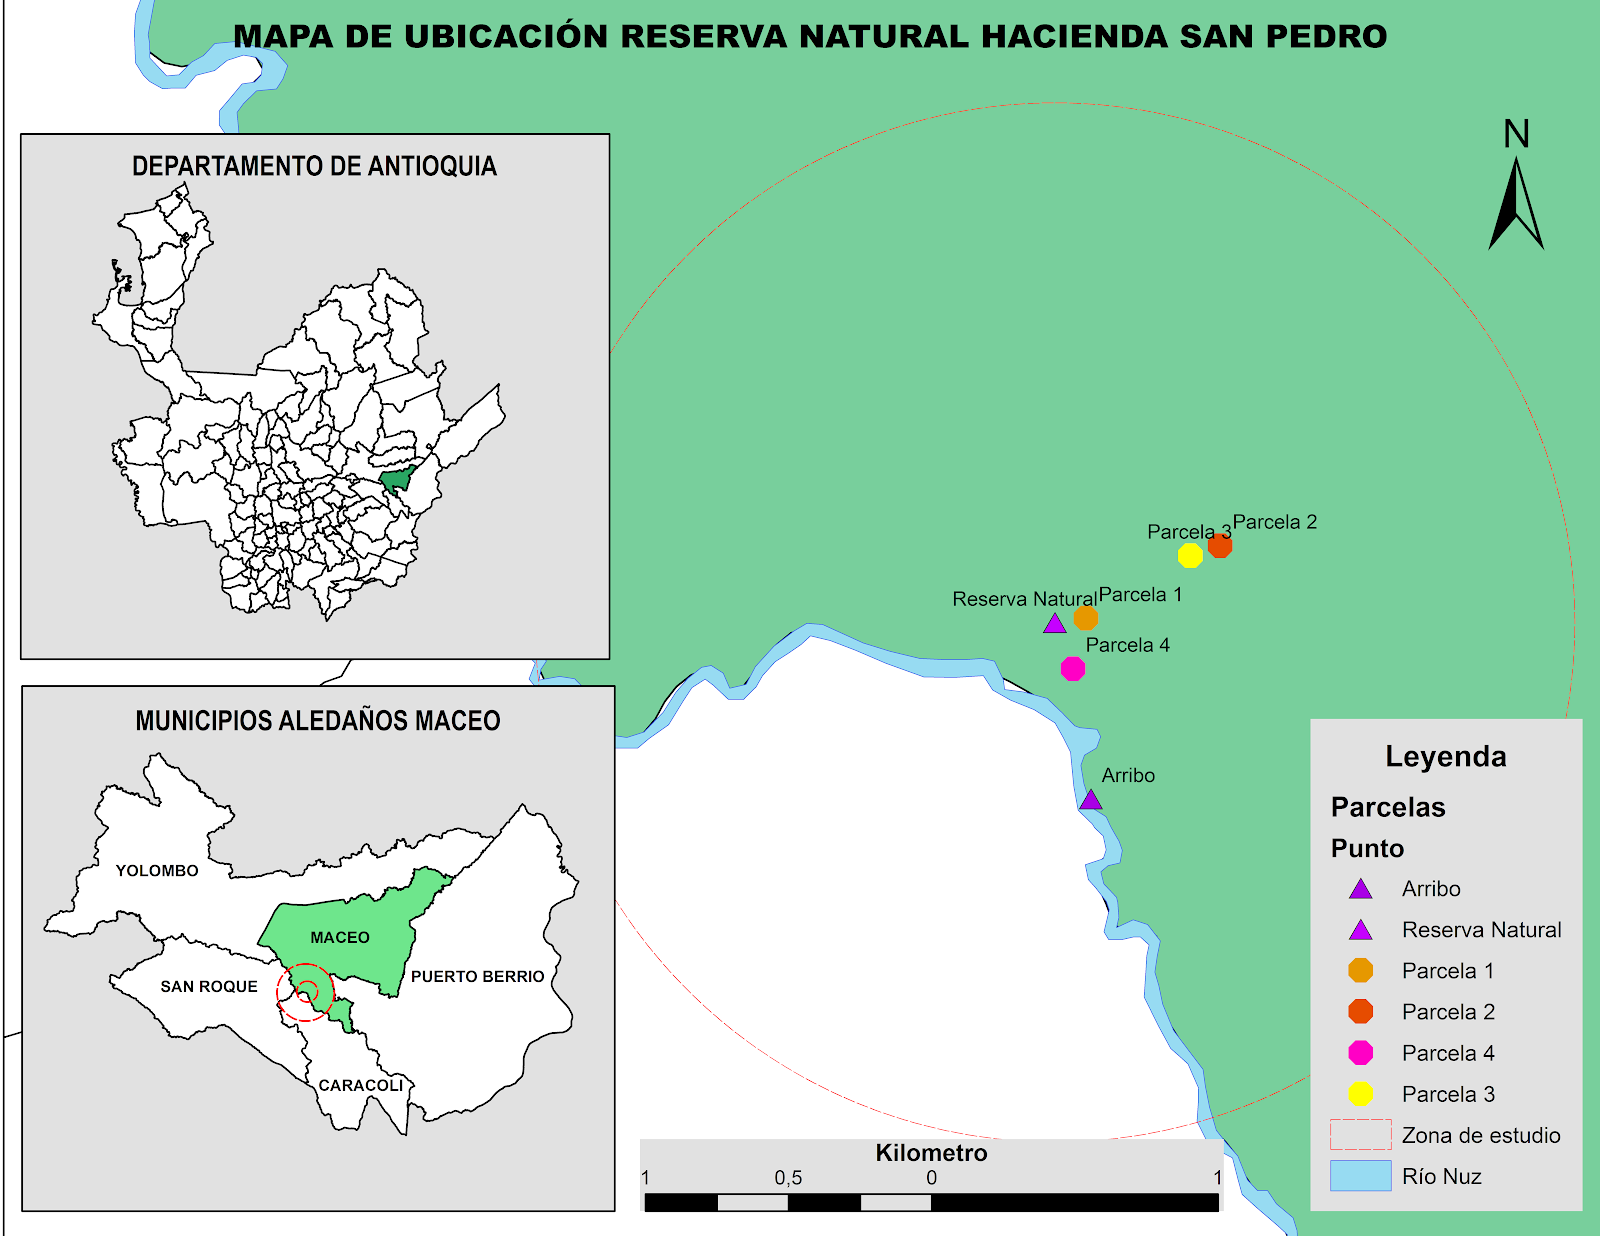
\includegraphics[width= 0.7\textwidth]{area.png}
  \caption{Reserva Natural Hacienda San Pedro}
\end{figure}

El desarrollo del presente trabajo se dio en dos etapas las cuales se
describen a continuación:

\hypertarget{levantamiento-de-informaciuxf3n}{%
\subsubsection{1) Levantamiento de
información}\label{levantamiento-de-informaciuxf3n}}

Para la recolección de la información se procedió a establecer áreas
determinadas para cada parcela estudiada de acuerdo con condiciones como
la topografía y logísticas que permitieran el desarrollo del trabajo. Se
centró la recolección de la información en especies de plantas comunes
en las diferentes parcelas; para el caso del presente análisis se
trabajaron las especies Vismia Macrophylla y Jacaranda Copaia. Las áreas
de las parcelas y especificaciones se se relacionan en la \textbf{Table
1}

\begin{table}

\caption{\label{tab:unnamed-chunk-1}Areas de parcelas trabajadas}
\centering
\begin{tabular}[t]{r|r|l|l|l}
\hline
Parcela & Área (m2) & Figura geométrica & Dimensiones (m) & Sucesión\\
\hline
1 & 500 & Circunferencia & r = 12,62 & SS1\\
\hline
2 & 324 & Cuadrado & 18 x 18 & SS3\\
\hline
3 & 450 & Rectángulo & 30 x 15 & SS2\\
\hline
4 & 800 & Rectángulo & 40 x 20 & SS1\\
\hline
\end{tabular}
\end{table}

Una vez establecidas las parcelas se procedió a recolectar la
información de las correspondientes especies, para esto se realizó una
categorización de estas en tres tamaños
los cuales fueron Brinzales, Latizales y Fustales; dicha descripción se
presenta en la \textbf{Table 2}

\begin{table}

\caption{\label{tab:unnamed-chunk-2}Catregorias de especies}
\centering
\begin{tabular}[t]{l|l|l}
\hline
Categoría vegetación & Tamaño DAP (cm) & Altura (m)\\
\hline
Brinzales & <5 & 1 - 1,5\\
\hline
Latizales & 5-10 & NA\\
\hline
Fustales & >10 & NA\\
\hline
\end{tabular}
\end{table}

Posterior al montaje de cada una de las parcelas se procedió a medir la
altura \((m)\) y el diamétro a la altura del pecho\(DAP \ (cm)\) de las 
especies que se estudiaron. Para
el registro de los datos se utilizó la \texttt{App\ Memento} en la cual
se tuvo en cuenta la corrección por pendiente para el caso de la
categoría de fustales, en latizales no se hizo
corrección por pendiente y para brinzales se realizó la
respectiva medición con la cinta métrica. En cada una de las parcelas se
observaron características bióticas y abióticas como fueron
vegetación dominante, cobertura, características del sustrato, topografía y
perturbaciones (antrópicas o naturales).

Otro de los aspectos que se tomó en cuenta en la recolección de los
datos fue la fotografía bajo el dosel de cada una de las parcelas
con el objetivo de realizar la respectiva caracterización de radiación
que pasa a través del sotobosque y entender la relación que tiene con el
estado de sucesión de las parcelas. También, se tomaron dichas
fotografías para observar la relación que guarda la radiación con los
hábitos de crecimiento de las especies que se analizaron.

\hypertarget{procesamiento-de-los-datos-recolectados}{%
\subsubsection{2) Procesamiento de los datos
recolectados}\label{procesamiento-de-los-datos-recolectados}}

\hypertarget{a-ajuste-del-modelo}{%
\paragraph{a) Ajuste del modelo}\label{a-ajuste-del-modelo}}

Se ajustó un modelo que describiera la altura en función del \(DAP\). El
modelo biológicamente correcto presenta comúnmente una forma sigmoidea
con un punto de inflexión en la parte inferior de los datos o bien forma
cóncava sin punto de inflexión aparente \citep{huan}, esto sugiere
modelos no lineales que ajusten el comportamiento esperado; por
experiencia se sabe que hay modelos alométricos que describen lo ya
mencionado, es el caso del modelo Weibull y Michaelis Menten, estos se
escogieron para el ajuste, pues son funciones que siguen la ontogenia
natural. Para hacerlos, se tuvo que ordenar los datos, algunos de estos
no eran lógicos, se encontró DAP del orden de \(2cm\) o menos con
alturas de \(96 m\) lo cual no es posible, se halló que todos los datos
no superan \(50 m\) de altura, excepto algunos con el problema descrito,
se hace un filtro de Altura \(< \ 50 m\), con esto, se ajustan los
modelos para las dos especies en cuestión.

\hypertarget{b-procesamiento-de-fotografuxedas-del-dosel}{%
\paragraph{b) Procesamiento de fotografías del
dosel}\label{b-procesamiento-de-fotografuxedas-del-dosel}}

El dosel influye en la cantidad de radiación del bosque dependiendo de
la incidencia directa o indirecta que llegue al ecosistema.
La penetración de la radiación depende de la localización, del tamaño,
la arquitectura y altura del dosel. La radiación lumínica disponible se
estimó mediante fotografías realizadas en campo, las imágenes se
procesaron con el software \texttt{imagenJ}. Este programa convierte las
fotos en imágenes binarias de blancos y negros \textbf{Fig.2}, de esta manera
se puede obtener el porcentaje blancos en cada fotografía asumiendo
este como el porcentaje de radiación que atraviesa el dosel \textbf{Table 3}.

\begin{figure}[h]
  \centering
  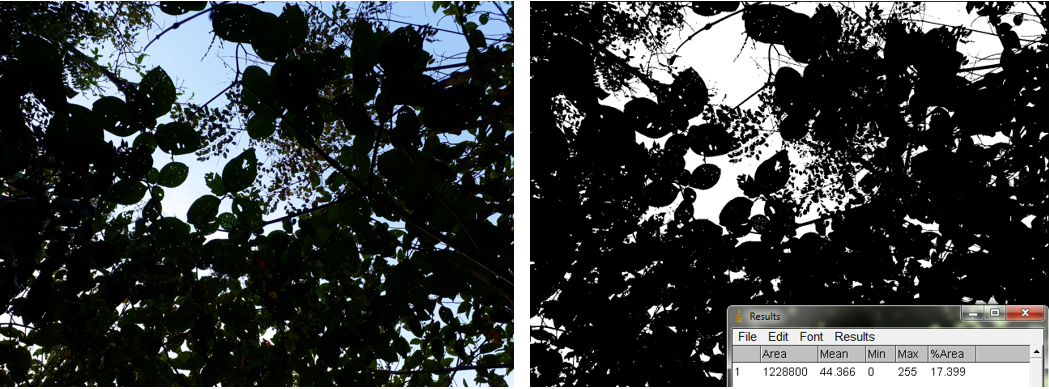
\includegraphics[width= 0.7\textwidth]{ima2.png}
  \caption{Conversión de imagenes a blancos y negros}
\end{figure}

\hypertarget{resultados-y-discusiuxf3n}{%
\section{Resultados y Discusión}\label{resultados-y-discusiuxf3n}}

En la \textbf{Fig.3} se muestra el modelo escogido (Michaelis Menten),
el modelo Weibull a pesar de tener un \(RSE\) de \(2.67\) con un \(AIC\)
de \(873.76\) frente al Michaelis Menten \(RSE\) de \(2.70\) con un
\(AIC\) de \(876.90\), no se puede escoger como el mejor modelo pues
gráficamente tiende disminuir la altura a medida que aumenta el
\(DAP \ > \ 25cm\) lo cual no tiene sentido, lo normal sería un tendencia
asintótica a medida que aumenta el DAP; por esta razón se elige al
modelo de Michaelis Menten como el que ajusta mejor a los datos,
pues sigue la tendencia natural para representar la variación de la
altura con respecto al estado de sucesión relacionado con cada parcela.
El ajuste ``predice'' de buena manera el comportamiento del sitio, pues
muestra cómo las categorias de vegetación (brinzales y latizales) tienen una
pendiente de la recta tangente mayor, lo cual se puede interpretar como
la tasa de cambio de la altura en función del DAP, es de esperarse que
el crecimiento en etapas tempranas sea rápido, \citep{lasky} informaron
tendencias de crecimiento-diversidad más fuertes y positivas durante la
sucesión temprana, seguidas de tendencias de crecimiento-diversidad
débiles y negativas en rodales más antiguos, es decir, que a una edad
temprana y por ende una sucesión primaria donde es común encontrar
brinzales y algunos latizales, la tasa de cambio de la altura será mayor
que en otros estados, esto puede ser causa de que el crecimiento es
producto de diversos factores bióticos y abióticos que interactúan
sobre un árbol y sobre el bosque \citep{forest}. Hay diversos factores
que influyen en el crecimiento de los árboles en este estudio, sólo se
esboza someramente el efecto de la luz.


\begin{figure}

{\centering 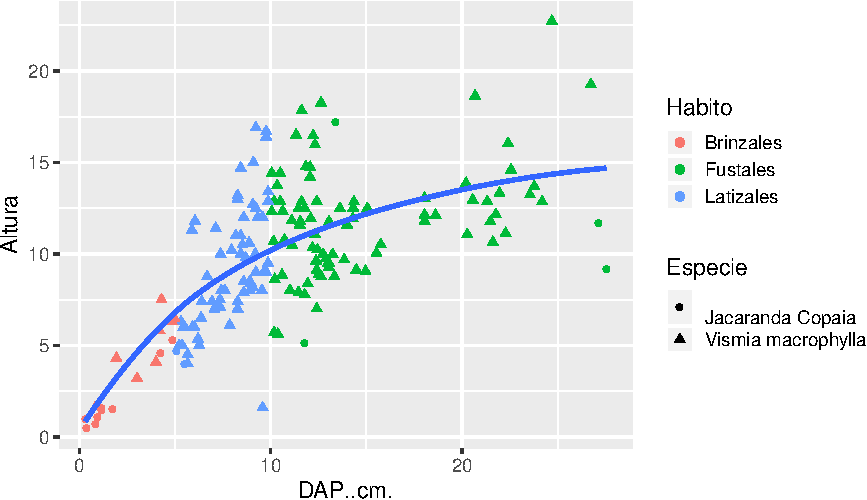
\includegraphics[width=0.7\textwidth]{report_ecology_files/figure-latex/unnamed-chunk-6-1} 

}

\caption{Modelo Michaelis Menten especie-habito}\label{fig:unnamed-chunk-6}
\end{figure}

Los diferentes estados de sucesión del bosque que presenta cada parcela
con sus condiciones de sitio (suelo y clima) mostraron que \emph{Jacaranda Copaia} esté presente en mayor cantidad en la parcela 3 con un estado
de sucesión SS2 y ausente en la parcela 1 con estado de secesión SS1
donde por la escasa vegetación arbórea hay mayor disponibilidad de luz y
así las especies heliófilas como \emph{Jacaranda Copaia} deberían
ser más prósperas, aunque es necesario aclarar que varios individuos de
esta especie podrían no ser representados en la toma de datos de la
parcela 1, lo que no sucede en la parcela 4 que también tiene un estado
de sucesión SS1 y si cuenta con individuos de dicha especie, esto se
puede otorgar a qué \emph{Jacaranda Copaia} es una especie heliófita y
pionera en la regeneración de bosques \citep{tapia}, por lo mismo se
explica que esté presente en mayor cantidad en la parcela 3 con estado
de sucesión SS2 donde dominan la especies heliófitas de rápido
crecimiento gracias al gran porcentaje de radiación que atraviesa el
dosel (\textbf{Table 3}).

\begin{table}

\caption{\label{tab:unnamed-chunk-7}Porcentaje de radiación que atraviesa el dosel}
\centering
\begin{tabular}[t]{r|l|l|l}
\hline
Parcela & Sucesión & \%R que atraviesa dosel & \%R que No atraviesa dosel\\
\hline
1 & SS1 & 17.4 & 82.6\\
\hline
2 & SS3 & 8.92 & 91, 08\\
\hline
3 & SS2 & 17, 15 & 82, 85\\
\hline
4 & SS1 & 17, 38 & 82, 62\\
\hline
\end{tabular}
\end{table}

De acuerdo con la \textbf{Fig.3} se puede evidenciar la poca cantidad de
individuos de \emph{Jacaranda Copaia} en comparación con la especie
\emph{Vismia Macrophylla} que se encuentra en todas las parcelas y en
mayor cantidad. La Reserva Natural Hacienda San Pedro, tiene
predominio de áreas con bosque secundario en regeneración natural
\citep{sala}, esto se demuestra mediante la cantidad de individuos que se
encuentran de \emph{Vismia Macrophylla} en la mayoría de sus parcelas.
Además, el sitio históricamente ha tenido intervenciones agrícolas de
ganadería y café, por lo cual es de esperarse este tipo de vegetación
predominante, esto podría explicarse por que el uso de la tierra de alta
intensidad puede reducir en gran medida la capacidad de recuperación de
los ecosistemas al empobrecer el banco de semillas del suelo, agotar los
nutrientes para el ciclado y compactar el suelo, así como al aumentar la
distancia de los bosques maduros que son las principales fuentes de
diversidad \citep{grubb, hooper, pic}, así mismo, la tierra sometida a
sucesivos sucesos de incendios a menudo engendra bosques secundarios
dominados por las especies pioneras del género Vismia (Hypericaceae)
\citep{jak}

Para mostrar el número de individuos por hectárea de las dos especies
estudiadas se presenta \textbf{Fig.4}, en la cual se evidencia que
\emph{Vismia Macrophylla} presenta una mayor cantidad de individuos en
la categoría de latizales y fustales , es decir, con DAP mayores a 5 cm,
para todas las parcelas. Por otro lado, se observa que \textbf{Jacaranda
Copaia} presenta la mayor cantidad de individuos con un DAP menor a 5 cm
(categoría brinzales). Para el caso de la parcela 2, se observa que si
bien \emph{Jacaranda Copaia} alcanza una baja cantidad de individuos
en la categoría de fustales (DAP mayores a 10 cm), es decir árboles
antiguos, con esto es suficiente para dispersar semillas y obtener de
esta manera en la categoría de brinzales (DAP menores a 5 cm) árboles
jóvenes, un buen número de individuos por hectárea para esta especie, lo
que vendría siendo la regeneración del bosque en dicha parcela; lo mismo
ocurren en la parcela 3 donde se tiene una menor cantidad de
individuos en las categorías latizales y fustales y gran cantidad en la
categoría de Brinzales para dicha especie. Otro de los aspectos a
considerar es que en la parcela 2 se presenta el mayor estado de
sucesión (SS3), en la categoría de latizales no hay presencia de
\emph{Jacaranda Copaia}; esto se ve reflejado en los pocos individuos que
dominan el dosel de dicha especie y su regeneración, es decir mayor
cantidad en la categoría de Brinzales.

Con respecto a \emph{Vismia Macrophylla} se pueden hacer algunas
apreciaciones relacionadas con las parcelas 1 y 4. Como se ha mencionado
anteriormente, este género es uno de los pioneros en la regeneración de
un bosque, esto se ve reflejado en estas dos parcelas las cuales
presentan la mayoría de individuos asociados a esta especie (salvo
categoría brinzales para parcela 4); una de las posibles razones para
esta salvedad es que si bien las parcelas 1 y 4 se clasificaron bajo el
mismo estado de sucesión(SS1), la parcela 1 tenía un uso para la
ganadería un poco más reciente comparado con la parcela 4, lo que puede
estar relacionado con que al tener más perturbación en esta parcela no
es posible la adaptación inicial de \emph{Jacaranda Copaia}. Además
podría estar relacionado con el sitio de muestreo de la parcela 1,
debido a que estaba ubicada en una zona en límite con el uso
agropecuario, ya que podría imposibilitar la llegada de semillas de
\emph{Jacaranda Copaia} para su colonización, esto se puede presentar
por un efecto de borde para dicha parcela.


\begin{figure}

{\centering 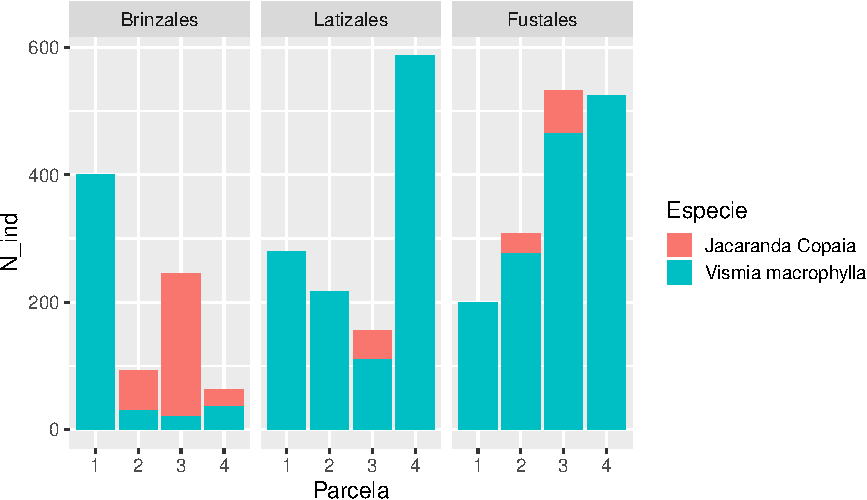
\includegraphics[width=0.7\textwidth]{report_ecology_files/figure-latex/unnamed-chunk-10-1} 

}

\caption{Relación número de individuos (Ha) y categoría de vegetación por parcela}\label{fig:unnamed-chunk-10}
\end{figure}

La forma y la disposición del dosel en las diferentes parcelas y sus
respectivos estados de sucesión dieron lugar a dos grupos de formaciones
significativas sobre la radiación disponible en el bosque. El primero de
ellos comprende las parcelas 1,3 y 4 que pertenecen a los estados de
sucesión SS1, SS2 Y SS1 respectivamente donde en las parcelas 1 y 4 se
puede encontrar presencia de pastos y escasa vegetación arbórea, la
parcela 3 cuenta con vegetación arbórea, con presencia de helechos y
especies heliófilas de rápido crecimiento. Es por eso que en este primer
grupo, la radiación incidente fue en promedio de \(17 \%\)
(\textbf{Table 3}) de radiación disponible, esto puede presentarse por
una baja densidad y tamaño en las copas de los árboles\citep{plateros}
lo que permite el paso de una mayor cantidad de luz al sotobosque. Por
otro lado en la parcela 2 perteneciente al estado de sucesión SS3 la
radiación disponible no superó el \(8 \%\) (\textbf{Table 3}) debido a
que en este estado de regeneración se pueden encontrar algunos árboles de
altura mayor a \(30 m\) es por esto que el dosel esta mas cerrado y no
permite un gran ingreso de radiación al interior del bosque, lo que
genera influencia en los procesos fisiológicos, morfológicos y
reproductivos de los organismos presentes bajo el dosel, favorecido así
a plantas epifitas y especies tolerantes a la sombra \citep{plateros}.
Por estos motivos se puede explicar la ausencia de \textbf{Jacaranda
Copaia} en esta parcela para la categoría de Latizales (\textbf{Fig.2}).

Otra de las características importantes para la parcela 2 es que al
presentar unas copas más cerradas en sus árboles se dan procesos de
acumulación de materia orgánica en forma de hojarasca lo cual permitirá
que en dicho estado de sucesión se mejoren las condiciones de
disponibilidad de nutrientes en el suelo, aumente la riqueza del banco
de semillas y se mejoren las condiciones de regeneración para la
consolidación del bosque. Caso contrario, ocurre con las parcelas 1, 3 y
4, que si bien presentan estados de sucesión diferentes tiene la
característica que no alcanzan ese cierre de copas necesario para
empezar a acumular materia orgánica por medio de la hojarasca y por este
motivo presentan especies que realizan un ciclado de nutrientes muy
eficiente para presentar un crecimiento más rápido en comparación con
las especies que ya están establecidas en la parcela 2 la cual se
explica en el modelo presentado.

\hypertarget{conclusiones}{%
\section{Conclusiones}\label{conclusiones}}

A mayor estado de sucesión del bosque menor es la cantidad de luz
disponible bajo el dosel y por ende menor la regeneración de plantas
Heliófilas.

El uso y actividades previas del suelo puede llegar a ser limitante en
la regeneración de un bosque y colonización de ciertas especies
(Jacaranda Copaia).

la poca disponibilidad de luz en el sotobosque dificulta el crecimiento
de especies Heliófitas.

%\showmatmethods


\bibliography{pinp}
\bibliographystyle{jss}



\end{document}

